\documentclass[aspectratio=169]{beamer}

\usepackage{amsmath,amssymb}
\usepackage{graphicx}
\usepackage{tikz}
\usepackage{listings}
\usetikzlibrary{positioning,calc,arrows.meta,fit}

% =========================
% Colors
% =========================
\definecolor{PKUDarkPurple}{RGB}{63,63,191}
\definecolor{PKULightPurple}{RGB}{170,170,225}
\definecolor{PKUGrayBg}{RGB}{255,255,255}
\definecolor{PKUTextBlue}{RGB}{45,45,190}
\definecolor{CodeGray}{RGB}{245,245,245}
\definecolor{dkgreen}{rgb}{0,0.5,0}
\definecolor{gray}{rgb}{0.4,0.4,0.4}
\definecolor{mauve}{rgb}{0.58,0,0.82}

% =========================
% Global style
% =========================
\setbeamercolor{background canvas}{bg=PKUGrayBg}
\setbeamercolor{normal text}{fg=black,bg=PKUGrayBg}
\setbeamercolor{frametitle}{fg=PKUTextBlue,bg=PKUGrayBg}

\setbeamerfont{normal text}{size=\fontsize{15pt}{18pt}\selectfont}
\setbeamerfont{frametitle}{size=\fontsize{15pt}{19pt}\selectfont,series=\bfseries}
\setbeamerfont{itemize/enumerate body}{size=\fontsize{12pt}{15pt}\selectfont}
\setbeamerfont{itemize/enumerate subbody}{size=\fontsize{11pt}{14pt}\selectfont}
\setbeamerfont{footline}{size=\fontsize{10pt}{12pt}\selectfont}

\setbeamercolor{itemize item}{fg=PKUDarkPurple}
\setbeamertemplate{navigation symbols}{}
\setbeamertemplate{items}[ball]

\setbeamertemplate{headline}{}
\setbeamertemplate{footline}{}

% =========================
% Code style
% =========================
\lstset{
  basicstyle=\ttfamily\footnotesize,
  backgroundcolor=\color{CodeGray},
  keywordstyle=\color{blue},
  commentstyle=\color{dkgreen},
  stringstyle=\color{mauve},
  showstringspaces=false,
  breaklines=true,
  frame=single,
  columns=fullflexible
}

% =========================
% Custom headline
% =========================
\newcommand{\makecustomheadline}{
\begin{tikzpicture}[remember picture,overlay]
    \fill[PKUDarkPurple]
        (current page.north west)
        rectangle
        ([xshift=.50\paperwidth,yshift=-0.35cm]current page.north west);

    \fill[PKULightPurple]
        ([xshift=.50\paperwidth]current page.north west)
        rectangle
        ([xshift=\paperwidth,yshift=-0.35cm]current page.north west);
\end{tikzpicture}
}

% =========================
% Custom footline
% =========================
\newcommand{\makecustomfootline}{
\begin{tikzpicture}[remember picture,overlay]
    \fill[PKUDarkPurple]
        (current page.south west)
        rectangle
        ([xshift=.33\paperwidth,yshift=0.42cm]current page.south west);

    \fill[PKULightPurple]
        ([xshift=.33\paperwidth]current page.south west)
        rectangle
        ([xshift=.67\paperwidth,yshift=0.42cm]current page.south west);

    \fill[PKULightPurple]
        ([xshift=.67\paperwidth]current page.south west)
        rectangle
        ([xshift=\paperwidth,yshift=0.42cm]current page.south west);

    \node[anchor=center, text=white, font=\small]
        at ([xshift=.165\paperwidth,yshift=0.21cm]current page.south west)
        {\textrm{huangxun@pku.edu.cn}};

    \node[anchor=center, text=white, font=\small]
        at ([xshift=.50\paperwidth,yshift=0.21cm]current page.south west)
        {AI Enabled Control Engineering};

    \node[anchor=center, text=black, font=\small]
        at ([xshift=.83\paperwidth,yshift=0.21cm]current page.south west)
        {2026 Summer};

    \node[anchor=center, text=black, font=\small]
        at ([xshift=.965\paperwidth,yshift=0.21cm]current page.south west)
        {\insertframenumber/\inserttotalframenumber};
\end{tikzpicture}
}

\addtobeamertemplate{background}{\makecustomheadline\makecustomfootline}{}

% =========================
% Placeholder figure
% =========================
\newcommand{\placeholderfig}[2]{
\begin{center}
\begin{tikzpicture}
    \draw[thick, rounded corners=4pt] (0,0) rectangle (8,#2);
    \node[align=center] at (4,{#2/2}) {\Large Placeholder Figure\\[3pt]\normalsize #1};
\end{tikzpicture}
\end{center}
}

% =========================
% Title info
% =========================
\title{\textcolor{PKUTextBlue}{AI Enabled Control Engineering}}
\author{\textcolor{blue}{Professor Xun Huang}}
\institute{
Aeronautics and Astronautics\\
College of Engineering\\
Peking University\\[0.25cm]
huangxun@pku.edu.cn\\
https://xunger99.github.io/xunger/
}
\date{}

\setbeamertemplate{title page}{
    \vspace{1.0cm}
    \begin{center}
        {\fontsize{18}{22}\selectfont\bfseries \inserttitle\par}
        \vspace{0.3cm}
        {\fontsize{15}{18}\selectfont Lecture 6: Rotary Inverted Pendulum Modeling, Hardware System Introduction, and STM32 Env Setup\par}
          \vspace{0.3cm}
        {\fontsize{15}{18}\selectfont \insertauthor\par}
        \vspace{0.15cm}
        {\fontsize{11}{13}\selectfont TA: Zhixiang Ju \quad Haozhe Wang\par}
        \vspace{0.4cm}
        {\fontsize{8}{11}\selectfont \insertinstitute\par}
    \end{center}
}

\begin{document}

% ---------------------------------
\begin{frame}
\titlepage
\end{frame}

% ---------------------------------
\begin{frame}{Recap}
\begin{itemize}
    \item Reinforcement learning overview.
    \vspace{0.3cm}
    \item Q-learning and why Q-tables fail for CartPole.
    \vspace{0.3cm}
    \item Deep Q-Network (DQN): replay buffer and target network.
    \vspace{0.3cm}
    \item Practical workflow of CartPole training and testing.
    \vspace{0.3cm}
\end{itemize}
\end{frame}

% ---------------------------------
\begin{frame}{Lecture 6}
\begin{itemize}
    \item Why move from CartPole to the rotary inverted pendulum.
    \vspace{0.3cm}
    \item Hardware system introduction:  motor, sensors, motor driver and STM32F446RE microcontroller.
    \vspace{0.3cm}
    \item Nonlinear dynamics modelling by the Lagrange method.
    \vspace{0.3cm}
    \item Arduino IDE setup, flashing and debugging for STM32F446RE.
    \vspace{0.3cm}
\end{itemize}
\end{frame}

% ---------------------------------
\begin{frame}{Why move from CartPole to the rotary inverted pendulum?}

CartPole is a very useful first benchmark, but it is still a software environment.

\vspace{0.3cm}
The rotary inverted pendulum is more suitable for the next stage because
\vspace{0.3cm}
\begin{itemize}
    \item it is a portable experimental platform,
    \vspace{0.3cm}
    \item it is nonlinear, coupled, and underactuated,
    \vspace{0.3cm}
\end{itemize}

\vspace{0.3cm}
So the course now moves from a toy benchmark to a real hardware system.

\end{frame}

% ---------------------------------
% ---------------------------------
\begin{frame}{From simulation to real hardware}

\begin{center}
\begin{tikzpicture}[>=Latex, node distance=3.5cm]

\node[
    draw,
    rounded corners,
    inner sep=2pt,
    minimum width=3.8cm,
    minimum height=2.4cm
] (sim) {
    \includegraphics[width=3.6cm,height=2.2cm,keepaspectratio]{cartpole.png}
};

\node[
    draw,
    rounded corners,
    inner sep=2pt,
    minimum width=4.6cm,
    minimum height=2.4cm,
    right=4.2cm of sim
] (real) {
    \includegraphics[width=4.4cm,height=2.2cm,keepaspectratio]{rip.png}
};

\node[below=0.15cm of sim] {CartPole};
\node[below=0.15cm of real] {Rotary Inverted Pendulum};

\draw[->, thick] (sim.east) -- node[above] {next} (real.west);

\end{tikzpicture}
\end{center}

The real system introduces several new issues:
\begin{itemize}
    \item sensors ,
    \item motor driver and PWM,
    \item embedded code,
    \item communication delay.
\end{itemize}

\end{frame}

% ---------------------------------
\begin{frame}{Overall hardware system}

\begin{columns}[T]
\column{0.52\textwidth}
\vspace{0.3cm}
Typical hardware modules:
\vspace{0.3cm}
\begin{itemize}
    \item rotary arm and vertical pendulum,
    \vspace{0.3cm}
    \item angle sensors,
    \vspace{0.3cm}
    \item DC motor and TB6612 driver,
    \vspace{0.3cm}
    \item STM32F446RE control board,
    \vspace{0.3cm}
    \item host computer for data logging.
    \vspace{0.3cm}
\end{itemize}

\column{0.44\textwidth}

\begin{center}
\includegraphics[width=1\textwidth]{倒立摆全套.png}
\end{center}

\end{columns}

\end{frame}
% ---------------------------------
\begin{frame}{Hardware architecture}

\begin{center}
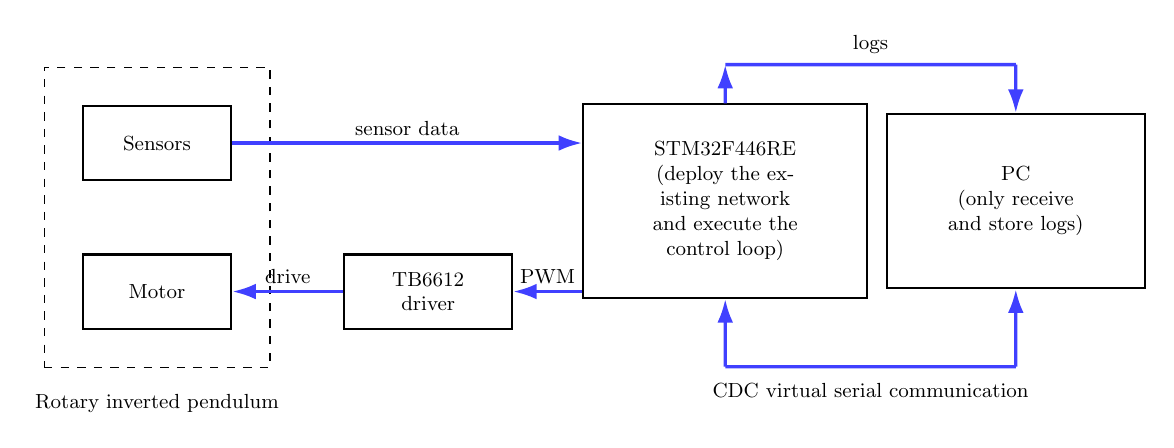
\begin{tikzpicture}[
    scale=0.82,
    transform shape,
    font=\small,
    >={Latex[length=3mm,width=2mm]},
    bluearrow/.style={->, draw=blue!75, very thick},
    blueplain/.style={-, draw=blue!75, very thick},
    smallbox/.style={draw, rectangle, thick, minimum width=2.3cm, minimum height=1.15cm, align=center},
    driverbox/.style={draw, rectangle, thick, minimum width=2.6cm, minimum height=1.15cm, align=center},
    stmbox/.style={draw, rectangle, thick, minimum width=4.4cm, minimum height=3.0cm, align=center, text width=3.9cm},
    pcbox/.style={draw, rectangle, thick, minimum width=4.0cm, minimum height=2.7cm, align=center, text width=3.5cm},
    dashedgroup/.style={draw, dashed, inner sep=0.48cm}
]

% 左侧实物系统
\node[smallbox] (sensor) at (0,0.8) {Sensors};
\node[smallbox] (motor)  at (0,-1.5) {Motor};
\node[dashedgroup, fit=(sensor)(motor)] (plantbox) {};
\node[below=0.28cm of plantbox] {Rotary inverted pendulum};

% 中间驱动与控制
\node[driverbox] (driver) at (4.2,-1.5) {TB6612\\driver};
\node[stmbox]    (stm)    at (8.8,-0.1) {STM32F446RE\\
(deploy the existing network\\
and execute the control loop)};

% 右侧 PC
\node[pcbox]     (pc)     at (13.3,-0.1) {PC\\
(only receive\\
and store logs)};

% Sensors -> STM
\draw[bluearrow] (sensor.east) -- (stm.west |- sensor.east);
\node[above] at ($(sensor.east)!0.5!(stm.west |- sensor.east)$) {sensor data};

% STM -> Driver
\draw[bluearrow] (stm.west |- driver.east) -- (driver.east);
\node[above] at ($(stm.west |- driver.east)!0.5!(driver.east)$) {PWM };

% Driver -> Motor
\draw[bluearrow] (driver.west) -- (motor.east);
\node[above] at ($(driver.west)!0.5!(motor.east)$) {drive};

% STM -> PC : logs（先上，再右，再下）
\coordinate (log_up_stm) at ($(stm.north)+(0,0.60)$);
\coordinate (log_up_pc)  at ($(pc.north)+(0,0.75)$);

\draw[bluearrow] (stm.north) -- (log_up_stm);
\draw[blueplain] (log_up_stm) -- (log_up_pc);
\draw[bluearrow] (log_up_pc) -- (pc.north);

\node[above=0.05cm] at ($(log_up_stm)!0.5!(log_up_pc)$) {logs};

% CDC 底部通信线：先画一条完全水平的主线，再分别竖直到两个框
\coordinate (cdc_left)  at ($(stm.south)+(0,-1.05)$);
\coordinate (cdc_right) at ($(pc.south)+(0,-1.2)$);

\draw[blueplain] (cdc_left) -- (cdc_right);
\draw[bluearrow] (cdc_left) -- (stm.south);
\draw[bluearrow] (cdc_right) -- (pc.south);

\node[below=0.14cm] at ($(cdc_left)!0.5!(cdc_right)$) {CDC virtual serial communication};

\end{tikzpicture}
\vspace{1.3cm}
\end{center}

\end{frame}



% ---------------------------------
% ---------------------------------
\begin{frame}{Motor}

The horizontal arm of the rotary inverted pendulum is driven by a DC motor with a gear reduction mechanism.



\begin{columns}[T]
\column{0.53\textwidth}

\textbf{Important motor parameters:}

\begin{itemize}
    \item \textbf{Rated voltage，Rated torque}

    \item \textbf{Stall torque}: maximum torque when the motor shaft is blocked.
    \item \textbf{Gear ratio}: ratio between motor-shaft rotation and output-shaft rotation.
\end{itemize}

\[
\omega_{\mathrm{out}} \approx \frac{\omega_{\mathrm{motor}}}{N},
\qquad
\tau_{\mathrm{out}} \approx \eta N\tau_{\mathrm{motor}} .
\]

\column{0.44\textwidth}

\textbf{Motor used in this system:}

\vspace{0.1cm}

\begin{center}
\begin{tabular}{l c}
\hline
Rated voltage & $12~\mathrm{V}$ \\
Rated current & $0.36~\mathrm{A}$ \\
Rated power & $4.32~\mathrm{W}$ \\
Rated torque & $0.06468~\mathrm{N\cdot m}$ \\
Stall current & $2.8~\mathrm{A}$ \\
Stall torque & $0.6468~\mathrm{N\cdot m}$ \\
No-load speed & $11000~\mathrm{rpm}$ \\
Output speed & $549\pm15~\mathrm{rpm}$ \\
\hline
\end{tabular}
\end{center}

\end{columns}
\end{frame}



\begin{frame}{Sensors}

The rotary inverted pendulum needs at least two angle-related measurements:

\begin{itemize}
    \item \textbf{arm angle} $\theta$,
    \item \textbf{pendulum angle} $\alpha$.
\end{itemize}

\vspace{0.3cm}
Typical implementations include
\begin{itemize}
    \item incremental encoder for the rotary arm,
    \item potentiometer or angle sensor for the pendulum.
\end{itemize}

\vspace{0.3cm}
From these measurements, we can further estimate the angular velocities
\[
\dot{\theta}, \qquad \dot{\alpha}
\]
using an observer.
\end{frame}


% ---------------------------------
% ---------------------------------
\begin{frame}{Sensor: Magnetic encoder}

A magnetic encoder measures rotation by detecting the change of magnetic field.

\vspace{0.25cm}
In this system, the motor tail is equipped with an incremental magnetic encoder.

\vspace{0.25cm}
When the motor shaft rotates, the magnetic encoder generates pulse signals.

\begin{itemize}
    \item The number of pulses reflects angular displacement.
    \item The pulse density reflects rotational speed.
    \item Two phase-shifted signals are used to determine direction.
\end{itemize}

\vspace{0.25cm}
Therefore, the encoder provides the basic measurement for the rotary arm angle:

\[
\text{encoder pulses}
\quad \Longrightarrow \quad
\theta .
\]

\end{frame}




% ---------------------------------
\begin{frame}{A/B phase signals and rotation direction}

An incremental encoder usually outputs two square-wave signals: A phase and B phase.



\begin{columns}[T]
\column{0.48\textwidth}

\begin{itemize}
    \item A phase and B phase have the same frequency.
    \item Their phase difference is approximately $90^\circ$.
    \item The leading phase determines the rotation direction.
\end{itemize}


For example:

\begin{itemize}
    \item if A phase leads B phase, the shaft rotates in one direction;
    \item if B phase leads A phase, the shaft rotates in the opposite direction.
\end{itemize}

\column{0.48\textwidth}

\begin{center}
\includegraphics[width=0.95\textwidth]{encoder_ab_phase.png}
\end{center}

\end{columns}

\end{frame}



% ---------------------------------
% ---------------------------------
\begin{frame}{From encoder pulses to rotation angle}

For this motor encoder, one motor-shaft revolution generates $13$ pulses.

\vspace{0.2cm}
The gear ratio is approximately $20:1$, meaning that the motor shaft rotates $20$ turns while the output shaft rotates $1$ turn.

\vspace{0.2cm}
Therefore, one output-shaft revolution generates $13 \times 20 = 260$ encoder pulse periods.

\vspace{0.2cm}
Because both A and B phases are counted on rising and falling edges, each pulse period provides four countable edges:

\[
260 \times 4 = 1040 .
\]

Thus,

\[
360^\circ \Longleftrightarrow 1040 \text{ counts},
\qquad
1 \text{ count} \Longleftrightarrow \frac{360^\circ}{1040}.
\]

\end{frame}


% ---------------------------------
\begin{frame}[fragile]{Firmware: counting encoder pulses}

In the STM32 firmware, the encoder A/B signals are connected to two external interrupt pins.  
The variable \texttt{g\_enc} stores the accumulated encoder count.

\vspace{0.12cm}

\begin{lstlisting}[language=C++]
static const int PIN_ENC_A = 2; 
static const int PIN_ENC_B = 3;
static volatile int32_t g_enc = 10000;
void setup() {
  pinMode(PIN_ENC_A, INPUT);
  pinMode(PIN_ENC_B, INPUT);
  attachInterrupt(digitalPinToInterrupt(PIN_ENC_A),
                  isr_enc_a, CHANGE);
  attachInterrupt(digitalPinToInterrupt(PIN_ENC_B),
                  isr_enc_b, CHANGE);
}
\end{lstlisting}


Each rising or falling edge of A/B triggers an interrupt, so the firmware can count pulses without continuously polling the encoder in the main loop.

\end{frame}


% ---------------------------------
\begin{frame}[fragile]{Firmware: direction judgment by A/B phase}

Whenever A or B changes its logic level, the corresponding interrupt service routine is called.



\begin{lstlisting}[language=C++]
void isr_enc_a() {
  bool A = digitalRead(PIN_ENC_A);
  bool B = digitalRead(PIN_ENC_B);
  if (A) g_enc += (B ? 1 : -1);
  else   g_enc += (B ? -1 : 1);
}
void isr_enc_b() {
  bool A = digitalRead(PIN_ENC_A);
  bool B = digitalRead(PIN_ENC_B);
  if (B) g_enc += (A ? -1 : 1);
  else   g_enc += (A ? 1 : -1);
}
\end{lstlisting}


This logic uses the current A/B levels to decide whether the count should increase or decrease.

\end{frame}

% ---------------------------------
\begin{frame}[fragile]{Firmware: from encoder count to arm angle}

When the command \texttt{GO} is received, the current encoder count is saved as the zero position:

\begin{lstlisting}[language=C++]
if (t == "GO") {
  noInterrupts();
  ENC_ZERO = g_enc; ...
  interrupts();
}
\end{lstlisting}

\vspace{0.15cm}
During each control tick, the firmware reads the current encoder count and converts it to the arm angle:

\begin{lstlisting}[language=C++]
int32_t enc = g_enc;
int32_t enc0 = ENC_ZERO;
g_theta_meas = (float)(enc - enc0) * THETA_SCALE;
\end{lstlisting}


\end{frame}

% ---------------------------------

% ---------------------------------
\begin{frame}[fragile]{Sensor: potentiometer}

The pendulum angle $\alpha$ is measured by a potentiometer connected to the STM32 analog input pin.

\vspace{0.2cm}

A potentiometer is a variable resistor. As the pendulum rotates, its resistance changes and produces a different analog voltage.

\vspace{0.2cm}

The STM32 ADC converts this analog voltage into a digital value.

\begin{lstlisting}[language=C++]
static const int PIN_POT = A0;
static const int32_t POT_MOD = 4096;

pinMode(PIN_POT, INPUT);
analogReadResolution(12);
\end{lstlisting}

\vspace{0.15cm}

Because 12-bit ADC is used, the raw potentiometer value is in the range

\[
0 \leq pot\_raw \leq 4095 .
\]

\end{frame}

% ---------------------------------
\begin{frame}[fragile]{From potentiometer value to pendulum angle}

Two calibration values are used in the firmware:

\begin{lstlisting}[language=C++]
static volatile int32_t POT_ZERO = 3090;      // upright position
static volatile int32_t POT_DOWN_RAW = 980;   // hanging-down position
\end{lstlisting}

\vspace{0.15cm}

The firmware reads the potentiometer in each control tick:

\begin{lstlisting}[language=C++]
int pot = analogRead(PIN_POT);
g_pot_raw = (int16_t)pot;

float alpha_branch = alphaFromPotRawBranchCutAtDown(pot);
g_alpha_meas = alpha_branch;
\end{lstlisting}


\[
\text{pendulum angle}
\rightarrow
\text{resistance}
\rightarrow
\text{voltage}
\rightarrow
pot\_raw
\rightarrow
\alpha .
\]

Here, \texttt{POT\_ZERO} corresponds to the upright position, and \texttt{POT\_DOWN\_RAW} is used to define the branch cut near the hanging-down position.

\end{frame}


% ---------------------------------
% ---------------------------------
\begin{frame}{Motor driver: TB6612}

The STM32 GPIO pins can only output low-power logic signals, so they cannot drive the DC motor directly.

\vspace{0.2cm}

The TB6612 motor driver is used as a power amplifier between the STM32 and the motor.



\begin{columns}[T]
\column{0.40\textwidth}

\begin{center}
\includegraphics[width=0.40\textwidth]{tb6612.png}
\end{center}

\column{0.50\textwidth}

\begin{itemize}
    \item \textbf{VM}: motor power supply.
    \item \textbf{VCC}: logic power supply.
    \item \textbf{GND}: common ground.
    \item \textbf{AO1, AO2}: motor output terminals.
\end{itemize}

\end{columns}

\vspace{0.1cm}

The TB6612 receives control signals from STM32 and provides higher current to the DC motor.

\end{frame}

% ---------------------------------
\begin{frame}[fragile]{TB6612 control pins in firmware}

For one DC motor, the STM32 mainly controls three types of signals:

\begin{itemize}
    \item \textbf{PWMA}: controls motor speed / torque level by PWM.
    \item \textbf{AI1, AI2}: control motor rotation direction.
    \item \textbf{STBY}: enables or disables the motor driver.
\end{itemize}

\vspace{0.15cm}

In the firmware, the corresponding pins are:

\begin{lstlisting}[language=C++]
static const int PIN_IN1  = 4;    // AI1
static const int PIN_IN2  = 5;    // AI2
static const int PIN_STBY = 7;    // STBY
static const int PIN_PWM  = 10;   // PWMA
\end{lstlisting}

\vspace{0.1cm}


\[
\text{STM32 PWM + direction}
\rightarrow
\text{TB6612}
\rightarrow
\text{DC motor}
\rightarrow
\text{rotary arm}.
\]

\end{frame}

% ---------------------------------
\begin{frame}{STM32F446RE development board}

\begin{columns}[T]
\column{0.42\textwidth}

\begin{center}
\includegraphics[width=0.75\textwidth]{STM32.png}
\end{center}

\column{0.64\textwidth}

The STM32F446RE is the real-time controller of the rotary inverted pendulum system.

\vspace{0.15cm}

Main tasks:

\begin{itemize}
    \item reading potentiometer by ADC;
    \item counting encoder pulses by external interrupts;
    \item generating PWM for the TB6612 driver;
    \item executing the control loop at a fixed frequency;
    \item communicating with the host computer through USB serial.
\end{itemize}

\vspace{0.15cm}

It connects sensing, computation, and actuation in the embedded control loop.

\end{columns}

\end{frame}


% ---------------------------------
\begin{frame}{Physical model of the rotary inverted pendulum}

\begin{columns}[T]
\column{0.46\textwidth}

\begin{center}
\includegraphics[width=1.25\textwidth]{axis.png}
\end{center}

\column{0.64\textwidth}

The rotary inverted pendulum consists of two rigid bodies:

\begin{itemize}
    \item horizontal rotary arm $OB$,
    \item vertical pendulum $BD$.
\end{itemize}




We define two generalized coordinates:

\[
q_1=\theta, \qquad q_2=\alpha .
\]

\begin{itemize}
    \item $\theta$: rotary arm angle;
    \item $\alpha$: pendulum angle relative to the upright position.
\end{itemize}

\end{columns}

\end{frame}


% ---------------------------------
\begin{frame}{State variables and modelling objective}

The system state is defined as

\[
x=
\begin{bmatrix}
\theta & \dot{\theta} & \alpha & \dot{\alpha}
\end{bmatrix}^{\top}.
\]


The goal of physical modelling is to derive the dynamic relationship between the motor input and the system motion:

\[
u \quad \Longrightarrow \quad
\theta,\ \dot{\theta},\ \alpha,\ \dot{\alpha}.
\]


The rotary inverted pendulum is

\begin{itemize}
    \item nonlinear,
    \item coupled,
    \item unstable around the upright equilibrium.
\end{itemize}


Therefore, we first build a nonlinear model and then linearize it around the upright position.

\end{frame}


% ---------------------------------
\begin{frame}{Lagrange equation}

The dynamics are derived using the Lagrange equation:

\[
\frac{d}{dt}
\left(
\frac{\partial T}{\partial \dot{q}_i}
\right)
-
\frac{\partial T}{\partial q_i}
+
\frac{\partial U}{\partial q_i}
=
Q_i,
\qquad i=1,2 .
\]

\vspace{0.25cm}

Here,

\begin{itemize}
    \item $T$ is the total kinetic energy,
    \item $U$ is the potential energy,
    \item $Q_i$ is the generalized force corresponding to $q_i$.
\end{itemize}

\vspace{0.25cm}

\[
q_1=\theta,
\qquad
q_2=\alpha .
\]

The two Lagrange equations give the coupled dynamics of the rotary arm and the pendulum.

\end{frame}




% ---------------------------------
\begin{frame}{Physical parameters and generalized forces}

\begin{center}
\renewcommand{\arraystretch}{1.18}
\begin{tabular}{c l}
\hline
Symbol & Meaning \\
\hline
$m_1$ & mass of the rotary arm $OB$ \\
$m_2$ & mass of the pendulum $BD$ \\
$l_1$ & distance from $O$ to the center of mass of arm $OB$ \\
$l_{21}$ & distance from joint $B$ to the center of mass of pendulum $BD$ \\
$I_{1z}$ & moment of inertia of arm $OB$ about its $z$ axis \\
$I_{2x}, I_{2y}, I_{2z}$ & moments of inertia of pendulum $BD$ about its body axes \\
$c_\theta$ & viscous damping coefficient of the rotary arm \\
$c_\alpha$ & viscous damping coefficient of the pendulum \\
$\tau$ & motor output torque \\
\hline
$Q_\theta = \tau - c_\theta \dot{\theta}$ & generalized force corresponding to $\theta$ \\
$Q_\alpha = -c_\alpha \dot{\alpha}$ & generalized force corresponding to $\alpha$ \\
\hline
\end{tabular}
\end{center}


\end{frame}


% ---------------------------------
\begin{frame}{Kinetic and potential energy}

The total kinetic energy is composed of the arm part and the pendulum part:

\[
T = T_{OB}+T_{BD}.
\]

\vspace{0.2cm}

The rotary arm contributes rotational kinetic energy:

\[
T_{OB}
=
\frac{1}{2}m_1 l_1^2 \dot{\theta}^2
+
\frac{1}{2}I_{1z}\dot{\theta}^2 .
\]

\vspace{0.2cm}

The pendulum contributes both translational and rotational kinetic energy:

\[
T_{BD}
=
\frac{1}{2}m_2 v_C^2
+
\frac{1}{2}
\left(
I_{2x}\dot{\alpha}^2
+
I_{2y}\dot{\theta}^2\sin^2\alpha
+
I_{2z}\dot{\theta}^2\cos^2\alpha
\right).
\]

\vspace{0.2cm}

The potential energy comes from gravity:

\[
U = -m_2 g l_{21}(1-\sin\phi).
\]

\end{frame}



% ---------------------------------
\begin{frame}{Nonlinear dynamic equations}

After substituting $T$ and $U$ into the Lagrange equations, the nonlinear coupled dynamics can be obtained.

\vspace{0.2cm}

Using $\alpha=\frac{\pi}{2}-\phi$, the equations can be written as

\[
\begin{aligned}
&
\left(
m_1l_1^2+I_{1z}+m_2l_1^2+m_2l_{21}^2\sin^2\alpha
+I_{2y}\cos^2\alpha+I_{2z}\sin^2\alpha
\right)\ddot{\theta}
\\
&\quad
+
(m_2l_1l_{21}\cos\alpha)\ddot{\alpha}
-
(m_2l_1l_{21}\sin\alpha)\dot{\alpha}^2
\\
&\quad
-
2\sin\alpha\cos\alpha
\left(
I_{2y}-I_{2z}-m_2l_{21}^2
\right)
\dot{\alpha}\dot{\theta}
=
Q_{\theta},
\end{aligned}
\]

\[
\begin{aligned}
&
-(m_2l_1l_{21}\cos\alpha)\ddot{\theta}
+
\sin\alpha\cos\alpha
\left(
I_{2z}-I_{2y}+m_2l_{21}^2
\right)\dot{\theta}^2
\\
&\quad
-
(I_{2x}+m_2l_{21}^2)\ddot{\alpha}
+
m_2gl_{21}\sin\alpha
=
Q_{\alpha}.
\end{aligned}
\]

\end{frame}




% ---------------------------------
\begin{frame}{Linearization around the upright equilibrium}

We linearize the nonlinear dynamics around the upright equilibrium:

\[
\theta = 0, 
\qquad
\alpha = 0 .
\]

\vspace{0.2cm}

Near the upright position, the small-angle approximations are

\[
\sin\alpha \approx 0,
\qquad
\cos\alpha \approx 1,
\qquad
\dot{\alpha}^2 \approx 0,
\qquad
\dot{\theta}^2 \approx 0 .
\]

\vspace{0.2cm}

After neglecting higher-order nonlinear terms, the nonlinear equations become

\[
\left(m_1l_1^2+I_{1z}+m_2l_1^2+I_{2y}\right)\ddot{\theta}
+
m_2l_1l_{21}\ddot{\alpha}
=
Q_\theta ,
\]

\[
-m_2l_1l_{21}\ddot{\theta}
-
\left(I_{2x}+m_2l_{21}^2\right)\ddot{\alpha}
+
m_2gl_{21}\alpha
=
Q_\alpha .
\]

\end{frame}


% ---------------------------------
\begin{frame}{Linearized model}

Define four constants:

\[
C_1=m_1l_1^2+I_{1z}+m_2l_1^2+I_{2y},
\qquad
C_2=m_2l_1l_{21},
\]

\[
C_3=I_{2x}+m_2l_{21}^2,
\qquad
C_4=m_2gl_{21}.
\]



Then the linearized dynamics can be written compactly as

\[
C_1\ddot{\theta}+C_2\ddot{\alpha}=Q_\theta ,
\]

\[
-C_2\ddot{\theta}-C_3\ddot{\alpha}+C_4\alpha=Q_\alpha .
\]


Where

\[
Q_\theta=\tau-c_\theta\dot{\theta},
\qquad
Q_\alpha=-c_\alpha\dot{\alpha}.
\]

\end{frame}


% ---------------------------------
\begin{frame}{State-space form}



After solving the two linearized second-order equations for $\ddot{\theta}$ and $\ddot{\alpha}$, the system can be written as

\[
\dot{x}=Ax+B\tau .
\]

\vspace{0.2cm}

The symbolic form is

\[
\frac{d}{dt}x=
\begin{bmatrix}
0 & 1 & 0 & 0 \\
0 & d_1 & a_1 & d_2 \\
0 & 0 & 0 & 1 \\
0 & d_3 & a_2 & d_4
\end{bmatrix}x
+
\begin{bmatrix}
0 \\ b_1 \\ 0 \\ b_2
\end{bmatrix}\tau .
\]

\vspace{0.1cm}



\end{frame}

% ---------------------------------
\begin{frame}{State-space form}

For the state vector
\[
x=
\begin{bmatrix}
\theta & \dot{\theta} & \alpha & \dot{\alpha}
\end{bmatrix}^{\top},
\]
the linearized model can be written as

\[
\dot{x}
=
\begin{bmatrix}
0 & 1 & 0 & 0 \\
0 & d_1 & a_1 & d_2 \\
0 & 0 & 0 & 1 \\
0 & d_3 & a_2 & d_4
\end{bmatrix}x
+
\begin{bmatrix}
0 \\ b_1 \\ 0 \\ b_2
\end{bmatrix}\tau.
\]

\vspace{-0.4cm}

where

\[
a_1=-\frac{C_2C_4}{C_1C_3-C_2^2},
\quad
a_2=\frac{C_1C_4}{C_1C_3-C_2^2},
\quad
b_1=\frac{C_3}{C_1C_3-C_2^2},
\quad
b_2=-\frac{C_2}{C_1C_3-C_2^2},
\]

\[
d_1=-\frac{C_3c_\theta}{C_1C_3-C_2^2},
\quad
d_2=\frac{C_2c_\alpha}{C_1C_3-C_2^2},
\quad
d_3=\frac{C_2c_\theta}{C_1C_3-C_2^2},
\quad
d_4=-\frac{C_1c_\alpha}{C_1C_3-C_2^2}.
\]

\end{frame}

% ---------------------------------
\begin{frame}{From motor torque to PWM command}

The mechanical model uses motor torque $\tau$ as the input, but the real system sends a PWM command $u$ through STM32 and TB6612.

\vspace{0.2cm}

Therefore, we need a DC motor model to connect the implemented command to the physical torque:

\[
u \quad \Longrightarrow \quad \tau .
\]

\vspace{0.2cm}

For a DC motor,

\[
V_{\mathrm{emf}}=k_i\omega,
\qquad
I=\frac{V_s-V_{\mathrm{emf}}}{R},
\qquad
\tau=k_t I .
\]

\vspace{0.2cm}

where $V_{\mathrm{emf}}$ is the back electromotive force, $\omega$ is motor angular velocity, $V_s$ is the applied voltage, $R$ is armature resistance, $I$ is motor current, and $k_t,k_i$ are motor constants.

\end{frame}

% ---------------------------------
\begin{frame}{PWM-to-torque relation}

The motor voltage is approximately proportional to the PWM command:

$
V_s = k_u u .
$



Substituting this into the DC motor model gives

\[
\tau
=
k_t\frac{V_s-k_i\omega}{R}
=
\frac{k_t k_u}{R}u
-
\frac{k_t k_i}{R}\omega .
\]



Therefore,

\[
\tau
=
K_u u
-
K_\omega \dot{\theta},
\]

where

\[
K_u=\frac{k_t k_u}{R},
\qquad
K_\omega=\frac{k_t k_i}{R}.
\]




\end{frame}

% ---------------------------------
% ---------------------------------
\begin{frame}{Substituting PWM input into the state-space model}

Before considering the motor electrical model, the linearized mechanical model is

\[
\dot{x}
=
A_{\tau}x+B_{\tau}\tau ,
\]

where

\[
A_{\tau}
=
\begin{bmatrix}
0 & 1 & 0 & 0 \\
0 & d_1 & a_1 & d_2 \\
0 & 0 & 0 & 1 \\
0 & d_3 & a_2 & d_4
\end{bmatrix},
\qquad
B_{\tau}
=
\begin{bmatrix}
0 \\ b_1 \\ 0 \\ b_2
\end{bmatrix}.
\]

From the previous slide,

\[
\tau=K_u u-K_\omega\dot{\theta}.
\]

Therefore,

\[
\dot{x}
=
A_{\tau}x
+
B_{\tau}
\left(
K_u u-K_\omega\dot{\theta}
\right).
\]

\end{frame}


% ---------------------------------
\begin{frame}{PWM-input state-space model}

Since the state vector is

\[
x=
\begin{bmatrix}
\theta & \dot{\theta} & \alpha & \dot{\alpha}
\end{bmatrix}^{\top},
\]

the term \(\dot{\theta}\) is the second state variable.


Thus, the back-EMF term \(-K_\omega B_{\tau}\dot{\theta}\) is absorbed into the second column of the state matrix:

\[
\dot{x}
=
A_1x+B_1u,
\]

where

\[
A_1
=
\begin{bmatrix}
0 & 1 & 0 & 0 \\
0 & d_1-K_\omega b_1 & a_1 & d_2 \\
0 & 0 & 0 & 1 \\
0 & d_3-K_\omega b_2 & a_2 & d_4
\end{bmatrix},
\qquad
B_1
=
\begin{bmatrix}
0 \\ K_u b_1 \\ 0 \\ K_u b_2
\end{bmatrix}.
\]


\end{frame}

% ---------------------------------
\begin{frame}{State-space form}

After substituting the physical parameters, the final linearized model is

\[
\dot{x}(t)=A_1x(t)+B_1u(t),
\]

where \(u(t)\) is the motor PWM command, and

\[
A_1=
\begin{bmatrix}
0 & 1 & 0 & 0 \\
0 & -11.3205 & -49.9955 & 0.4820 \\
0 & 0 & 0 & 1 \\
0 & 16.9206 & 171.2602 & -1.6510
\end{bmatrix},
\qquad
B_1=
\begin{bmatrix}
0 \\
0.8171 \\
0 \\
-1.2213
\end{bmatrix}.
\]

\vspace{0.2cm}

This model describes the local dynamics of the rotary inverted pendulum near the upright equilibrium.

\end{frame} 

% ---------------------------------
\begin{frame}{Arduino IDE setup for STM32F446RE}

Arduino IDE can be used as a lightweight development environment for STM32F446RE.

\vspace{0.2cm}

The basic workflow is:

\begin{enumerate}
    \item install Arduino IDE 2,
    \item add the STM32 board package URL,
    \item install \texttt{STM32 MCU based boards},
    \item select the correct STM32F446RE board,
    \item choose the upload method,
    \item compile and upload the firmware.
\end{enumerate}

\vspace{0.2cm}

This allows us to write Arduino-style sketches while still running them on the STM32 microcontroller.

\end{frame}

% ---------------------------------
\begin{frame}[fragile]{Install STM32 board package}

Open Arduino IDE:

\[
\texttt{File}
\rightarrow
\texttt{Preferences}
\rightarrow
\texttt{Additional Boards Manager URLs}
\]



Add the STM32duino package index URL:

\begin{lstlisting}[language=bash]
https://github.com/stm32duino/BoardManagerFiles/raw/main/package_stmicroelectronics_index.json
\end{lstlisting}



Then open:

\[
\texttt{Tools}
\rightarrow
\texttt{Board}
\rightarrow
\texttt{Boards Manager}
\]



Search for

\begin{lstlisting}[language=bash]
STM32 MCU based boards
\end{lstlisting}

and install the package.

\end{frame}

% ---------------------------------
\begin{frame}{Select the STM32F446RE board}

After installing the STM32 board package, select the board in Arduino IDE.

\vspace{0.2cm}

For the STM32F446RE Nucleo board, the typical selection path is:

\[
\texttt{Tools}
\rightarrow
\texttt{Board}
\rightarrow
\texttt{STM32 MCU based boards}
\rightarrow
\texttt{Nucleo-64}
\]

\vspace{0.2cm}

Then select the board part number:

\[
\texttt{Board part number}
\rightarrow
\texttt{Nucleo F446RE}
\]



Other useful settings are usually:

\begin{itemize}
    \item \textbf{Upload method}: \texttt{OpenOCD STLink} .
    \item \textbf{Port}: select the USB serial port of the board.
   
\end{itemize}

\end{frame}


% ---------------------------------
\begin{frame}[fragile]{Upload firmware to STM32F446RE}

Connect the STM32F446RE board to the computer through USB.





\begin{enumerate}
    \item select the correct board , board part number and upload method,
    \item select the correct port,
    
    \item click \textbf{Verify} to compile and click \textbf{Upload} to flash the firmware.
\end{enumerate}



A minimal test program is:

\begin{lstlisting}[language=C++]
void setup() {
  pinMode(LED_BUILTIN, OUTPUT);
}
void loop() {
  digitalWrite(LED_BUILTIN, HIGH);
  delay(500);
  digitalWrite(LED_BUILTIN, LOW);
  delay(500);
}
\end{lstlisting}

\end{frame}


% ---------------------------------
\begin{frame}[fragile]{Serial monitor test}

After uploading the firmware, we can use Serial Monitor to check communication.



Open:

\[
\texttt{Tools}
\rightarrow
\texttt{Serial Monitor}
\]



Set the baud rate to the same value used in the firmware, for example:

\begin{lstlisting}[language=C++]
void setup() {
  Serial.begin(115200);
}
void loop() {
  Serial.println("STM32 serial OK");
  delay(500);
}
\end{lstlisting}

\vspace{0.15cm}

If the setup is correct, the Serial Monitor should repeatedly print:

\begin{lstlisting}[language=bash]
STM32 serial OK
\end{lstlisting}

\end{frame}

% ---------------------------------
\begin{frame}{Flashing and debugging checklist}

If upload or serial communication fails, check the following items:

\begin{itemize}
    \item Is the STM32 board package installed?
    \item Is \texttt{Nucleo F446RE} selected as the board part number?
    \item Is the correct upload method selected?
    \item Is the correct USB port selected?
    \item Is the USB cable a data cable rather than a charging-only cable?
    \item Is the Serial Monitor baud rate the same as \texttt{Serial.begin()}?
    \item Is another program already occupying the serial port?
\end{itemize}

\vspace{0.2cm}



\end{frame}

% ---------------------------------
\begin{frame}{Summary}

In this lecture, we moved from a software benchmark to a real rotary inverted pendulum platform.

\vspace{0.2cm}

\begin{itemize}
    \item \textbf{Hardware system.}
   

    \item \textbf{Sensing and actuation.}
    
    \item \textbf{Physical modelling.}
    
    \item \textbf{PWM-input state-space model.}
    the motor torque model was combined with the mechanical model to obtain
    \[
    \dot{x}(t)=A_1x(t)+B_1u(t),
    \]
    where \(u(t)\) is the PWM command.

    \item \textbf{STM32 development workflow.}
   
\end{itemize}

\end{frame}

\end{document}